\documentclass[tikz,border=4pt]{standalone}
\usepackage{amsmath,amssymb}

\usetikzlibrary{arrows.meta,positioning,automata,shapes,shapes.misc,calc,decorations.pathmorphing,decorations.markings,angles,quotes,patterns,mindmap,matrix,knots,hobby,trees}
\tikzset{->-/.style={decoration={markings, mark=at position 0.5 with {\arrow{Stealth}}}, postaction={decorate}}}
\begin{document}
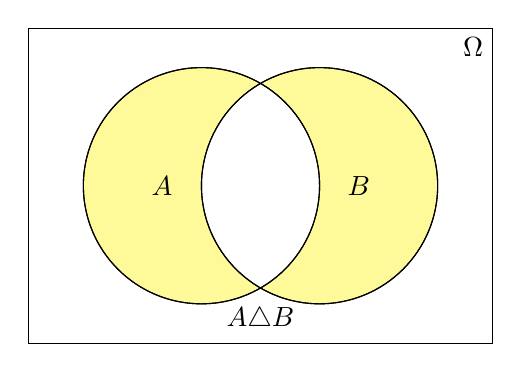
\begin{tikzpicture}
\draw[fill=yellow!40, even odd rule] (0,0) circle (1.5) (1.5,0) circle (1.5);
\draw (0,0) circle (1.5) (1.5,0) circle (1.5);
\draw (-2.2,-2) rectangle (3.7,2) node[below left] {$\Omega$};
\node at (-0.5,0) {$A$}; \node at (2,0) {$B$}; \node at (0.75,-1.7) {$A \triangle B$};
\end{tikzpicture}
\end{document}
